\chapter{Firegex}\label{chap:firegex}

Firegex è un \gls{sdfw} innovativo e multifunzionale, ideato per essere avviato con 0 configurazioni in modo rapido e semplice, che agisce principalmente a livello applicativo per permettere un'analisi del traffico specifica e dettagliata per ogni servizio. Esistono al suo interno diversi moduli che permettono la creazione di filtri di diversa natura, in modo semplice, flessibile e quanto meno invasivo ed impattante sulle prestazioni della macchina, mantenendo sempre la massima priorità sulla disponibilità e la corretta funzionalità del servizio stesso.

Il contesto per cui è stato pensato è quello delle competizioni \gls{ctf} di tipo \gls{ad}, dove vi sono particolari esigenze (descritte nel Capitolo~\ref{chap:ctfad}), che Firegex cerca di soddisfare, semplificandone il suo utilizzo, e soprattutto fornendo soluzioni adattabili ai requisiti spesso fortemente dinamici dei servizi in gara. Nella Figura~\ref{fig:firegex_frontend} si mostra l'interfaccia grafica di Firegex.

\begin{figure}[H]
    \centering
    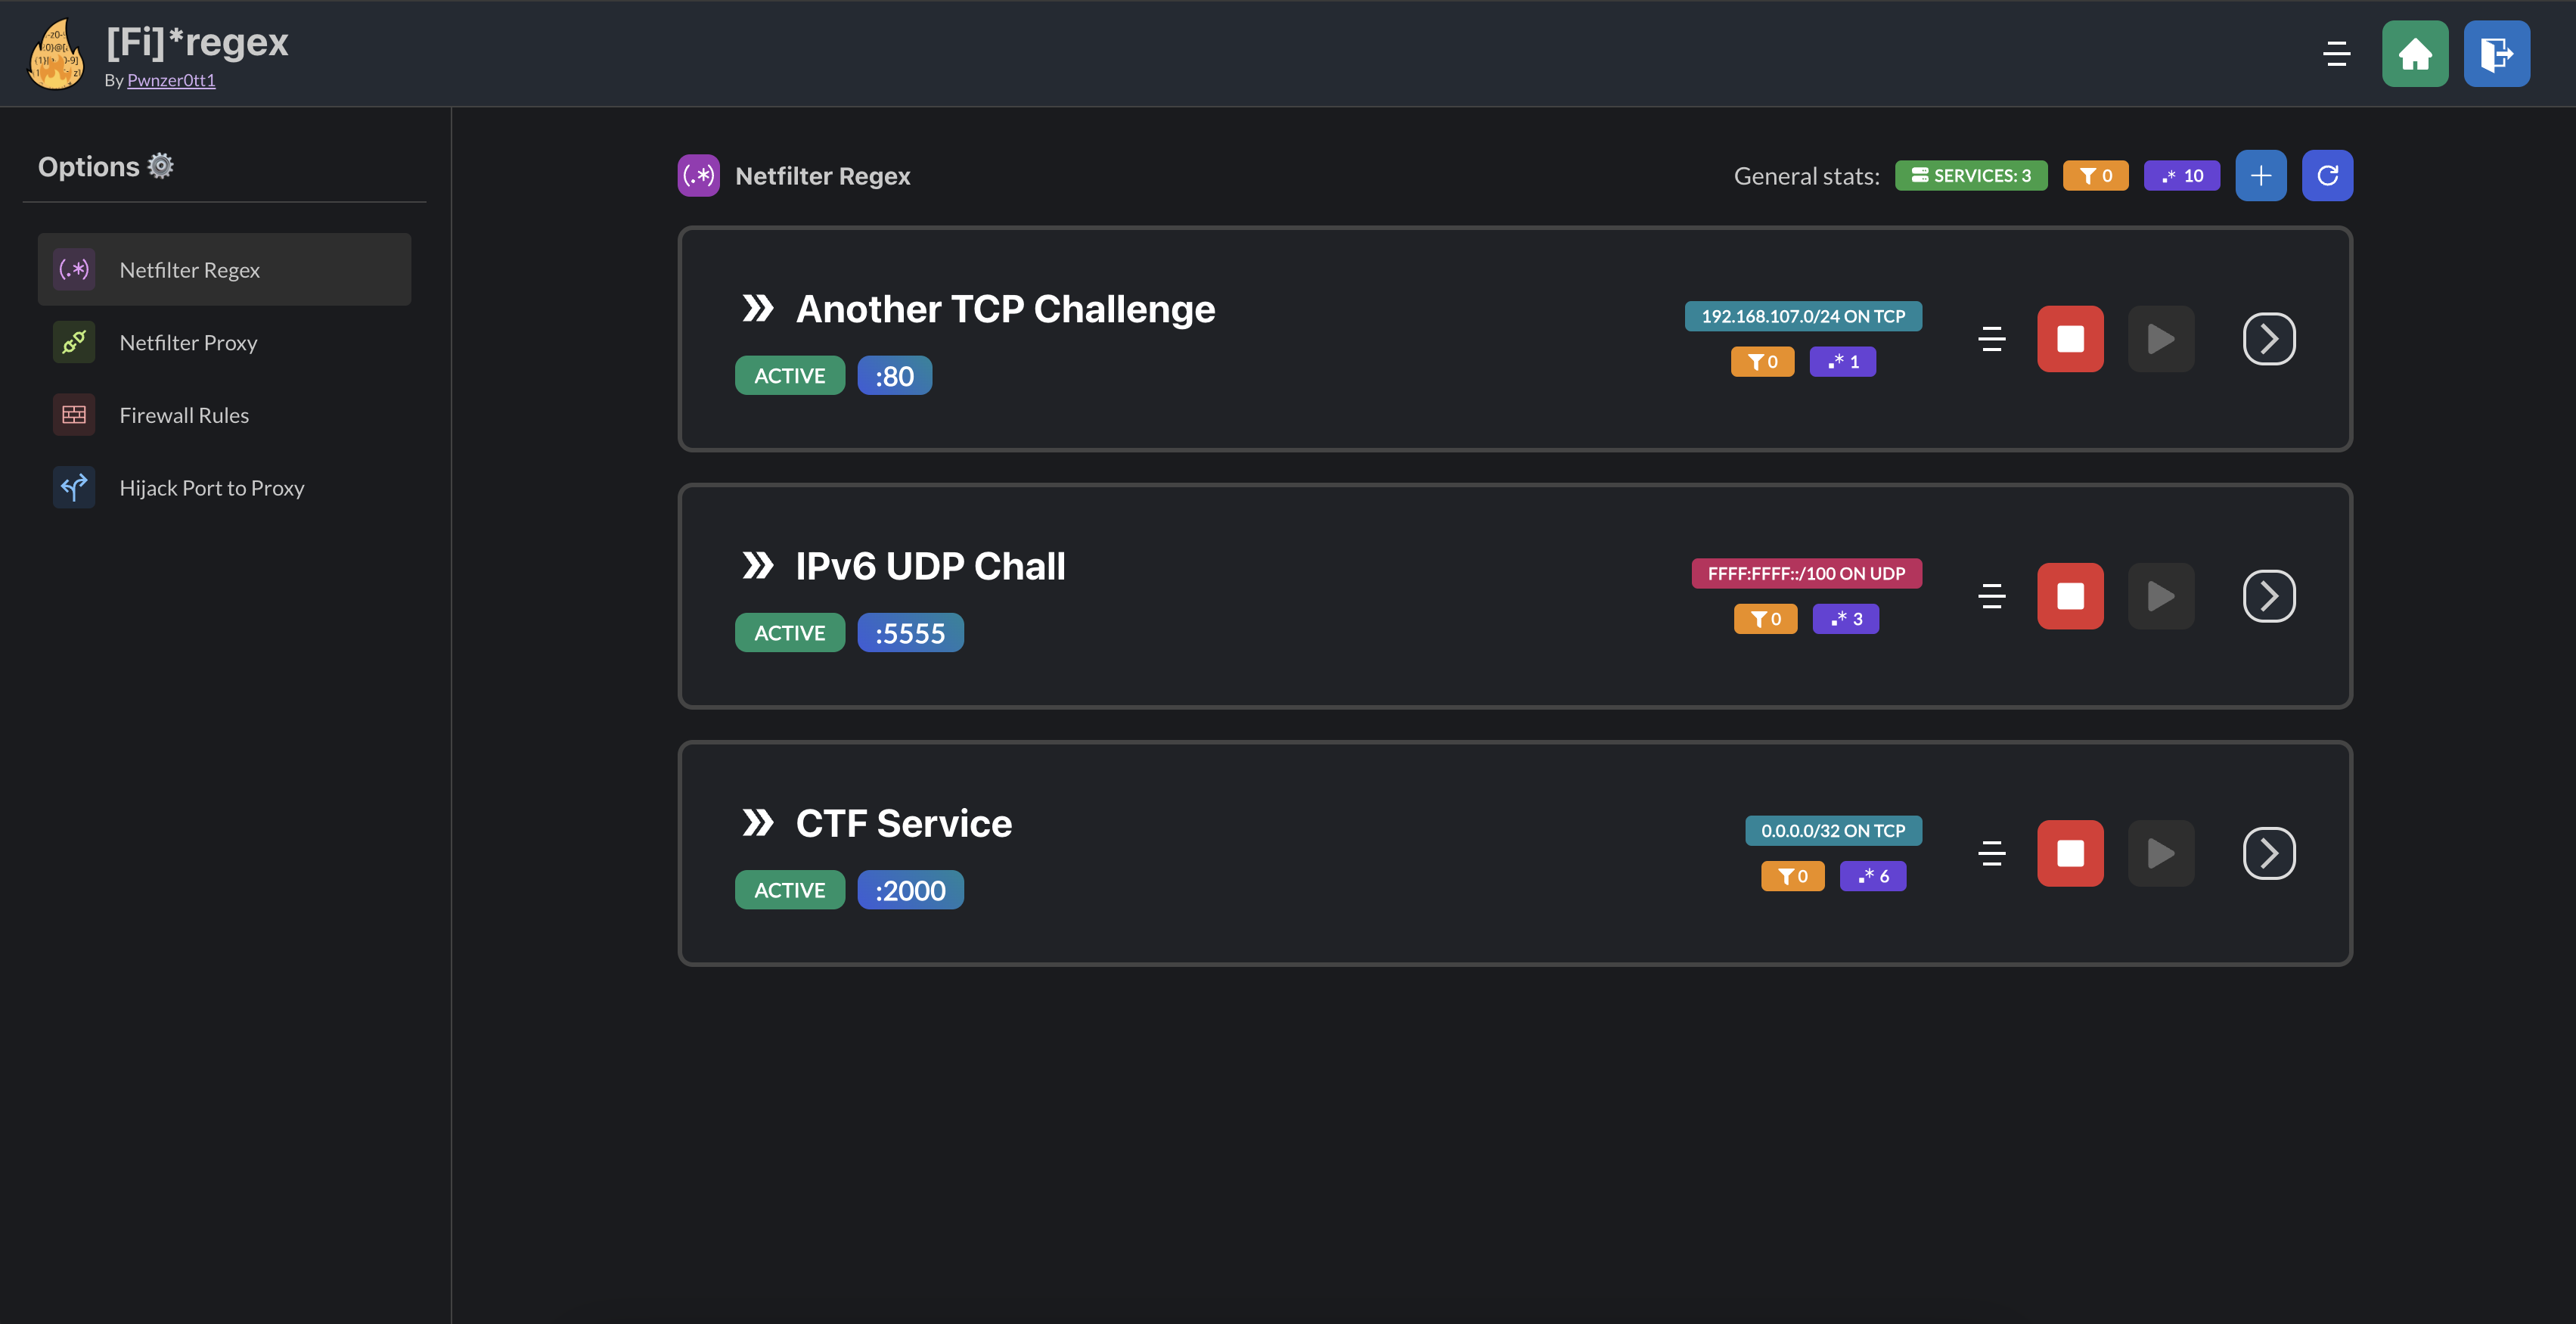
\includegraphics[width=1\textwidth]{images/chapter2/Firegex_Screenshot.png}
    \caption{Interfaccia grafica di Firegex.}\label{fig:firegex_frontend}
\end{figure}

\section{Perché nasce Firegex?}

Firegex (come detto in precedenza) nasce dal gruppo che ha affrontato la gara nazionale di Cyberchallenge\footcite{\url{https://cyberchallenge.it/}}{cyberchallenge} del 2022 al Politecnico di Bari\footcite{\url{https://www.poliba.it}}{poliba_website}, come un normale proxy con filtri basati sulle \gls{regex}, che col tempo si è evoluto aggiungendo nuove funzionalità sempre più efficienti, sicure e funzionali alla competizione stessa.

La sua necessità è nata proprio dalla mancanza di un sistema di difesa che fosse immediato da utilizzare, che non richiedesse configurazioni complesse per essere avviato, e che permettesse in maniera semplice di costruire dei filtri prontamente attivi, funzionanti e stabili.

Durante la sua progettazione, ci si è sempre più focalizzati su alcuni punti chiave che lo rendono unico rispetto ad altre soluzioni presenti:

\begin{itemize}
    \setlength{\itemsep}{1pt}
    \setlength{\parskip}{1pt}
    \item \textbf{Trasparenza totale:} La creazione di un proxy comporta una serie di cambiamenti sulla configurazione delle porte di rete esposte dai servizi, l'avvio e la gestione del processo del proxy stesso, e utilizzo di meccanismi di \textit{fallback} per ovviare ad eventuali problematiche. Queste complicanze erano solo parzialmente gestite inizialmente da firegex, ma con le nuove implementazioni è possibile applicare regole sul traffico senza cambiamenti nelle configurazione, grazie a particolari funzionalità utilizzate, disponibili nel kernel Linux, nascondendone però tutta la complessità gestita internamente per il loro corretto funzionamento;
    \item \textbf{Integrazione di tecnologie multiple:} Come già detto, Firegex utilizzava come unico meccanismo di filtraggio le \gls{regex}, che venivano applicate sui pacchetti di rete per individuare eventuali attacchi. Negli anni si è notato come questo approccio spesso potesse essere limitante, per cui sono stati implementati nuovi meccanismi e tecnologie di filtraggio aumentando la precisione con cui è possibile analizzare il traffico. La seguente tesi tratterà di una sua nuova funzionalità particolarmente flessibile denominata \texttt{\gls{nfproxy}};
    \item \textbf{Affidabilità e disponibilità:} In ambienti dove la continuità del servizio è critica, è fondamentale che il sistema di sicurezza non diventi un collo di bottiglia. Firegex è stato progettato per garantire un’elevata disponibilità, avendo meccanismi di \textit{fallback} applicati in caso di errori critici, e offrendo soluzioni rapide per il ripristino della configurazione in caso di errori e per il reset immediato dei filtri applicati;
    \item \textbf{Facilità di utilizzo:} Nelle \gls{ad} il tempo è una risorsa fondamentale: gli strumenti a disposizione per la gara non devono richiedere eccessivi tempi di configurazione e devono facilitare la risoluzione di problemi semplificando le eventuali fasi di troubleshooting, che possibilmente andrebbero evitate. L'obiettivo infatti è quello di focalizzare l'attenzione sull'individuazione di vulnerabilità, che rappresenta un necessità chiave nella competizione. Firegex è stato progettato per essere quanto meno dispersivo possibile, avere configurazioni semplici e guidate, un'interfaccia intuitiva, e gestire autonomamente tutte le problematiche legate alla gestione dei filtri e alla loro esecuzione.
\end{itemize}

\section{Confronto con altre soluzioni}

Firegex si distingue rispetto ad altre soluzioni presenti, come \gls{ctf} proxy\footcite{\url{https://github.com/ByteLeMani/ctf_proxy}}{ctf_proxy}, Nginx\footcite{\url{https://nginx.org/}}{nginx}, Suricata\footcite{\url{https://suricata.io/}}{suricata} o i \gls{ngfw} per diverse motivazioni mostrate nella Tabella~\ref{tab:firewall_compare}.

\renewcommand{\arraystretch}{2}
\begin{table}[H]
    \centering
    \setlength{\tabcolsep}{12pt}
    \begin{tabular}{|c|c|c|c|c|}
        \hline
        \begin{tabular}[c]{@{}c@{}} \textbf{Firewall} \end{tabular} &
        \begin{tabular}[c]{@{}c@{}} \textbf{0 Config Run}  \end{tabular} &
        \begin{tabular}[c]{@{}c@{}} \textbf{Easy use} \end{tabular} &
        \begin{tabular}[c]{@{}c@{}} \textbf{Easy Filter Add} \end{tabular} &
        \begin{tabular}[c]{@{}c@{}} \textbf{Flexible} \end{tabular} \\
        \hline
        \texttt{Firegex} &
        \begin{tabular}[c]{@{}c@{}} \color{Green}\faIcon[solid]{check-circle} \end{tabular} &
        \begin{tabular}[c]{@{}c@{}} \color{Green}\faIcon[solid]{check-circle} \end{tabular} &
        \begin{tabular}[c]{@{}c@{}} \color{Green}\faIcon[solid]{check-circle} \end{tabular} &
        \begin{tabular}[c]{@{}c@{}} \color{Green}\faIcon[solid]{check-circle} \end{tabular} \\
        \hline
        \texttt{Nginx} &
        \begin{tabular}[c]{@{}c@{}} \color{Orange}\faIcon[solid]{exclamation-circle} \end{tabular} &
        \begin{tabular}[c]{@{}c@{}} \color{Orange}\faIcon[solid]{exclamation-circle} \end{tabular} &
        \begin{tabular}[c]{@{}c@{}} \color{Orange}\faIcon[solid]{exclamation-circle} \end{tabular} &
        \begin{tabular}[c]{@{}c@{}} \color{Orange}\faIcon[solid]{exclamation-circle} \end{tabular} \\
        \hline
        \texttt{\gls{ctf} proxy} &
        \begin{tabular}[c]{@{}c@{}} \color{Red}\faIcon[solid]{times-circle} \end{tabular} &
        \begin{tabular}[c]{@{}c@{}} \color{Orange}\faIcon[solid]{exclamation-circle} \end{tabular} &
        \begin{tabular}[c]{@{}c@{}} \color{Orange}\faIcon[solid]{exclamation-circle} \end{tabular} &
        \begin{tabular}[c]{@{}c@{}} \color{Green}\faIcon[solid]{check-circle} \end{tabular} \\
        \hline
        \texttt{\gls{ngfw}} &
        \begin{tabular}[c]{@{}c@{}} \color{Red}\faIcon[solid]{times-circle} \end{tabular} &
        \begin{tabular}[c]{@{}c@{}} \color{Red}\faIcon[solid]{times-circle} \end{tabular} &
        \begin{tabular}[c]{@{}c@{}} \color{Orange}\faIcon[solid]{exclamation-circle} \end{tabular} &
        \begin{tabular}[c]{@{}c@{}} \color{Orange}\faIcon[solid]{exclamation-circle} \end{tabular} \\
        \hline
        \texttt{Suricata} &
        \begin{tabular}[c]{@{}c@{}} \color{Red}\faIcon[solid]{times-circle} \end{tabular} &
        \begin{tabular}[c]{@{}c@{}} \color{Orange}\faIcon[solid]{exclamation-circle} \end{tabular} &
        \begin{tabular}[c]{@{}c@{}} \color{Orange}\faIcon[solid]{exclamation-circle} \end{tabular} &
        \begin{tabular}[c]{@{}c@{}} \color{Orange}\faIcon[solid]{exclamation-circle} \end{tabular} \\
        \hline
    \end{tabular}
    \caption{Confronto tra le soluzioni per il firewall.}\label{tab:firewall_compare}
\end{table}
\renewcommand{\arraystretch}{1}

\begin{itemize}
    \setlength{\itemsep}{1pt}
    \setlength{\parskip}{1pt}
    \item \textbf{Nginx} è una soluzione molto flessibile ed affidabile, ma richiede configurazioni complesse e non permette di applicare filtri in maniera immediata e trasparente, ha necessità di cambiare porte e non supporta nativamente filtri più avanzati come quello trattato in questo lavoro di tesi. Non ha un'interfaccia grafica per la gestione delle regole;
    \item \textbf{\gls{ctf} proxy} è una soluzione fortemente flessibile, ma richiede la creazione di configurazioni e allo stesso modo necessita di cambiare porte ai servizi originali, inoltre a suo supporto non esiste un'interfaccia semplice da usare;
    \item I \textbf{\gls{ngfw}} offrono soluzioni estremamente affidabili, ben riconosciute nel settore, ma richiedono spesso configurazioni complesse e sono poco intuitivi da utilizzare. Pertanto il loro utilizzo risulta poco pratico per competizioni \gls{ctf}, nonostante rimangano le principali soluzioni applicate al di fuori di questo contesto;
    \item \textbf{Suricata} è una soluzione molto affidabile che offre un grado di flessibilità intermedio, ma pecca della mancanza di un'interfaccia semplice per il suo utilizzo, e richiede configurazioni per essere avviato.
\end{itemize}

\section{Integrazione con il networking su Linux}

In questa parte si descrive come Firegex si integra con il networking su Linux, in particolare con il framework Netfilter e le sue tabelle, che sono alla base della gestione del traffico di rete nel kernel Linux.
Il sistema target analizzato è basato su Linux dato il suo ampio utilizzo nelle competizioni \gls{ctf} ma anche in contesti di produzione, dove la flessibilità e le prestazioni sono fondamentali.

Quando un pacchetto di rete raggiunge l'interfaccia di una macchina Linux, viene avviato un processo di elaborazione articolato che attraversa diversi stadi nel kernel. Il pacchetto viene inizialmente ricevuto dall'hardware di rete e passato al driver della scheda, che lo trasferisce al sottosistema di rete del kernel attraverso interrupt o polling. Una volta nel kernel, il pacchetto attraversa il networking stack di Linux, passando per diverse fasi di elaborazione sequenziali.

Durante questo percorso, il framework Netfilter inserisce punti di intercettazione chiamati \textbf{hook} in momenti strategici del flusso di elaborazione. Questi hook, visibili nella Figura~\ref{fig:nftables_hooks}, permettono di eseguire operazioni personalizzate sui pacchetti in transito senza modificare il codice del kernel. I principali hook sono:

\begin{itemize}
    \setlength{\itemsep}{1pt}
    \setlength{\parskip}{1pt}
    \item \textbf{PREROUTING}: Eseguito immediatamente dopo la ricezione del pacchetto, prima delle decisioni di routing;
    \item \textbf{INPUT}: Attivato per pacchetti destinati al sistema locale;
    \item \textbf{FORWARD}: Gestisce pacchetti in transito verso altre destinazioni;
    \item \textbf{OUTPUT}: Elabora pacchetti generati localmente;
    \item \textbf{POSTROUTING}: Ultimo hook prima della trasmissione del pacchetto.
\end{itemize}

Ogni hook supporta l'esecuzione di regole con diverse \textbf{priorità} (prio), valori numerici che determinano l'ordine di esecuzione delle operazioni. Priorità negative vengono eseguite prima di quelle positive, permettendo un controllo granulare sulla sequenza di elaborazione. Ad esempio, operazioni di deframmentazione avvengono tipicamente a priorità -400, mentre il modulo \texttt{conntrack} opera a priorità -200.

\begin{figure}[H]
    \centering
    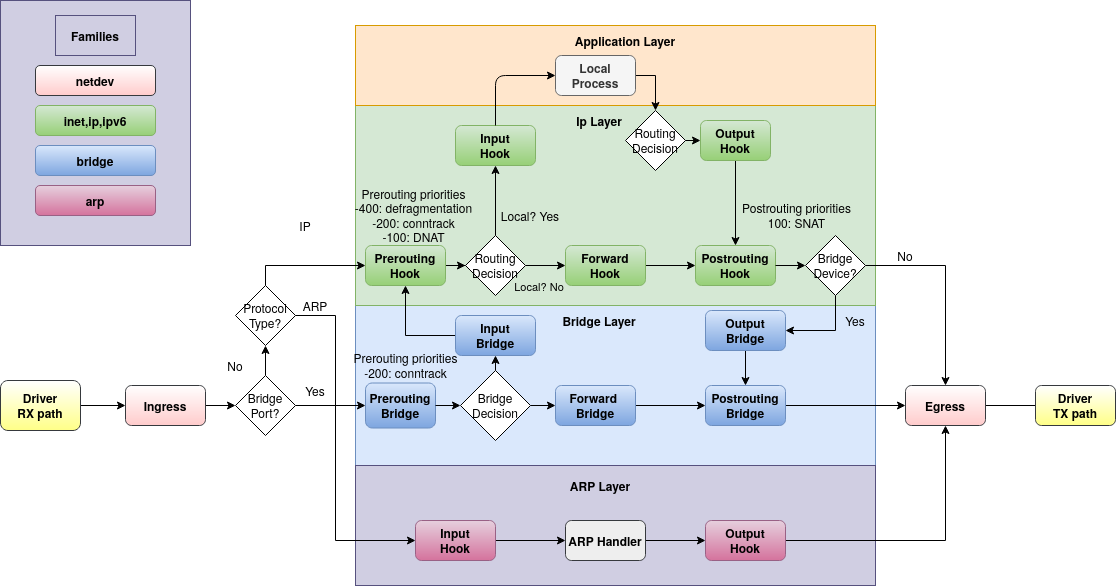
\includegraphics[width=0.98\textwidth]{images/chapter3/nf-hooks.png}
    \caption{Grafico degli hooks di Netfilter Tables.}\label{fig:nftables_hooks}
\end{figure}

Il framework \gls{nftables} rappresenta l'evoluzione moderna del sistema di filtraggio Linux, sostituendo il precedente sistema xtables utilizzato da iptables. Mentre iptables continua a essere ampiamente utilizzato per compatibilità, oggi impiega \gls{nftables} come backend, beneficiando delle sue prestazioni superiori e della sintassi semplificata. Questo processo di transizione porterà gradualmente all'eliminazione completa di xtables in favore dell'architettura più efficiente di \gls{nftables}.

Tra i moduli che operano negli hook di Netfilter, particolare rilevanza assume \texttt{conntrack}, responsabile del tracciamento delle connessioni. Questo modulo mantiene lo stato delle sessioni di rete, distinguendo tra nuove connessioni, traffico correlato a connessioni esistenti e pacchetti di risposta. Le informazioni gestite da \texttt{conntrack} sono fondamentali per l'implementazione di firewall stateful e per le operazioni di \gls{nat}.

\subsection{Netfilter Tables}

\gls{nftables} rappresenta il framework moderno per il filtraggio dei pacchetti e la gestione del traffico nelle distribuzioni Linux. Questo sistema permette di definire regole che vengono eseguite nei vari hook del percorso di elaborazione dei pacchetti, offrendo un controllo granulare e prestazioni ottimizzate.

In Firegex, \gls{nftables} costituisce il meccanismo fondamentale per intercettare e gestire il traffico di rete attraverso diverse modalità operative:

\begin{itemize}
    \item \textbf{Applicare regole di sicurezza:} Le regole di firewall tradizionali vengono implementate direttamente tramite \gls{nftables}, sfruttando le sue capacità native di filtraggio per bloccare, accettare o modificare il traffico in base a criteri specifici (indirizzi IP, porte, protocolli);

    \item \textbf{Reindirizzamento del traffico:} La funzionalità \texttt{\gls{porthijack}} utilizza le regole di \gls{nat} di \gls{nftables} per deviare trasparentemente il traffico da una porta a un'altra, permettendo l'inserimento di proxy intermedi senza modifiche alla configurazione dei servizi;

    \item \textbf{Integrazione con \gls{nfqueue}:} \gls{nftables} fornisce la base per l'attivazione del modulo \gls{nfqueue}, definendo quando e quali pacchetti devono essere trasferiti dallo spazio kernel allo spazio utente per elaborazioni avanzate.
\end{itemize}

\subsection{Netfilter Queue Module}

Il modulo \gls{nfqueue} rappresenta un'estensione specializzata del framework Netfilter che permette di trasferire pacchetti dallo spazio kernel allo spazio utente per elaborazioni complesse. Questo modulo opera come target delle regole \gls{nftables}, attivandosi quando una regola specifica il verdict \texttt{queue} su un pacchetto che attraversa uno degli hook di Netfilter.

Il funzionamento di \gls{nfqueue} segue un processo ben definito:

\begin{enumerate}
    \setlength{\itemsep}{1pt}
    \setlength{\parskip}{1pt}
    \item Una regola \gls{nftables} intercetta un pacchetto in uno degli hook del percorso di elaborazione;
    \item Se la regola specifica l'azione \texttt{queue}, il pacchetto viene trasferito a una coda numerata gestita da \gls{nfqueue};
    \item Un'applicazione userspace si registra per ricevere pacchetti da quella specifica coda;
    \item L'applicazione elabora il pacchetto e restituisce un verdict (ACCEPT, DROP, etc.), ed eventualmente modifica il pacchetto stesso;
    \item Il kernel applica il verdict ricevuto, continuando o interrompendo l'elaborazione del pacchetto.
\end{enumerate}

Questa architettura offre vantaggi significativi per Firegex:

\begin{itemize}
    \setlength{\itemsep}{1pt}
    \setlength{\parskip}{1pt}
    \item \textbf{Accesso completo ai pacchetti:} L'applicazione userspace riceve l'intero pacchetto, inclusi header di rete e trasporto, permettendo analisi approfondite e modifiche precise non possibili con proxy tradizionali;

    \item \textbf{Trasparenza totale:} L'intercettazione avviene a livello kernel senza richiedere modifiche alla configurazione dei servizi applicativi, che rimangono completamente ignari del processo di filtraggio;

    \item \textbf{Flessibilità nell'elaborazione:} Lo spazio utente permette l'implementazione di logiche complesse (parsing di protocolli, analisi con machine learning, integrazione con database) mantenendo la stabilità del kernel;

    \item \textbf{Controllo granulare del flusso:} La possibilità di modificare pacchetti e restituire verdict personalizzati offre un controllo fine sul comportamento della rete.
\end{itemize}

I moduli \texttt{\gls{nfregex}} e \texttt{\gls{nfproxy}} di Firegex sfruttano intensivamente questa architettura, registrandosi come listener su code \gls{nfqueue} specifiche e implementando le rispettive logiche di filtraggio in spazio utente.

\section{Architettura}

\begin{figure}[H]
    \centering
    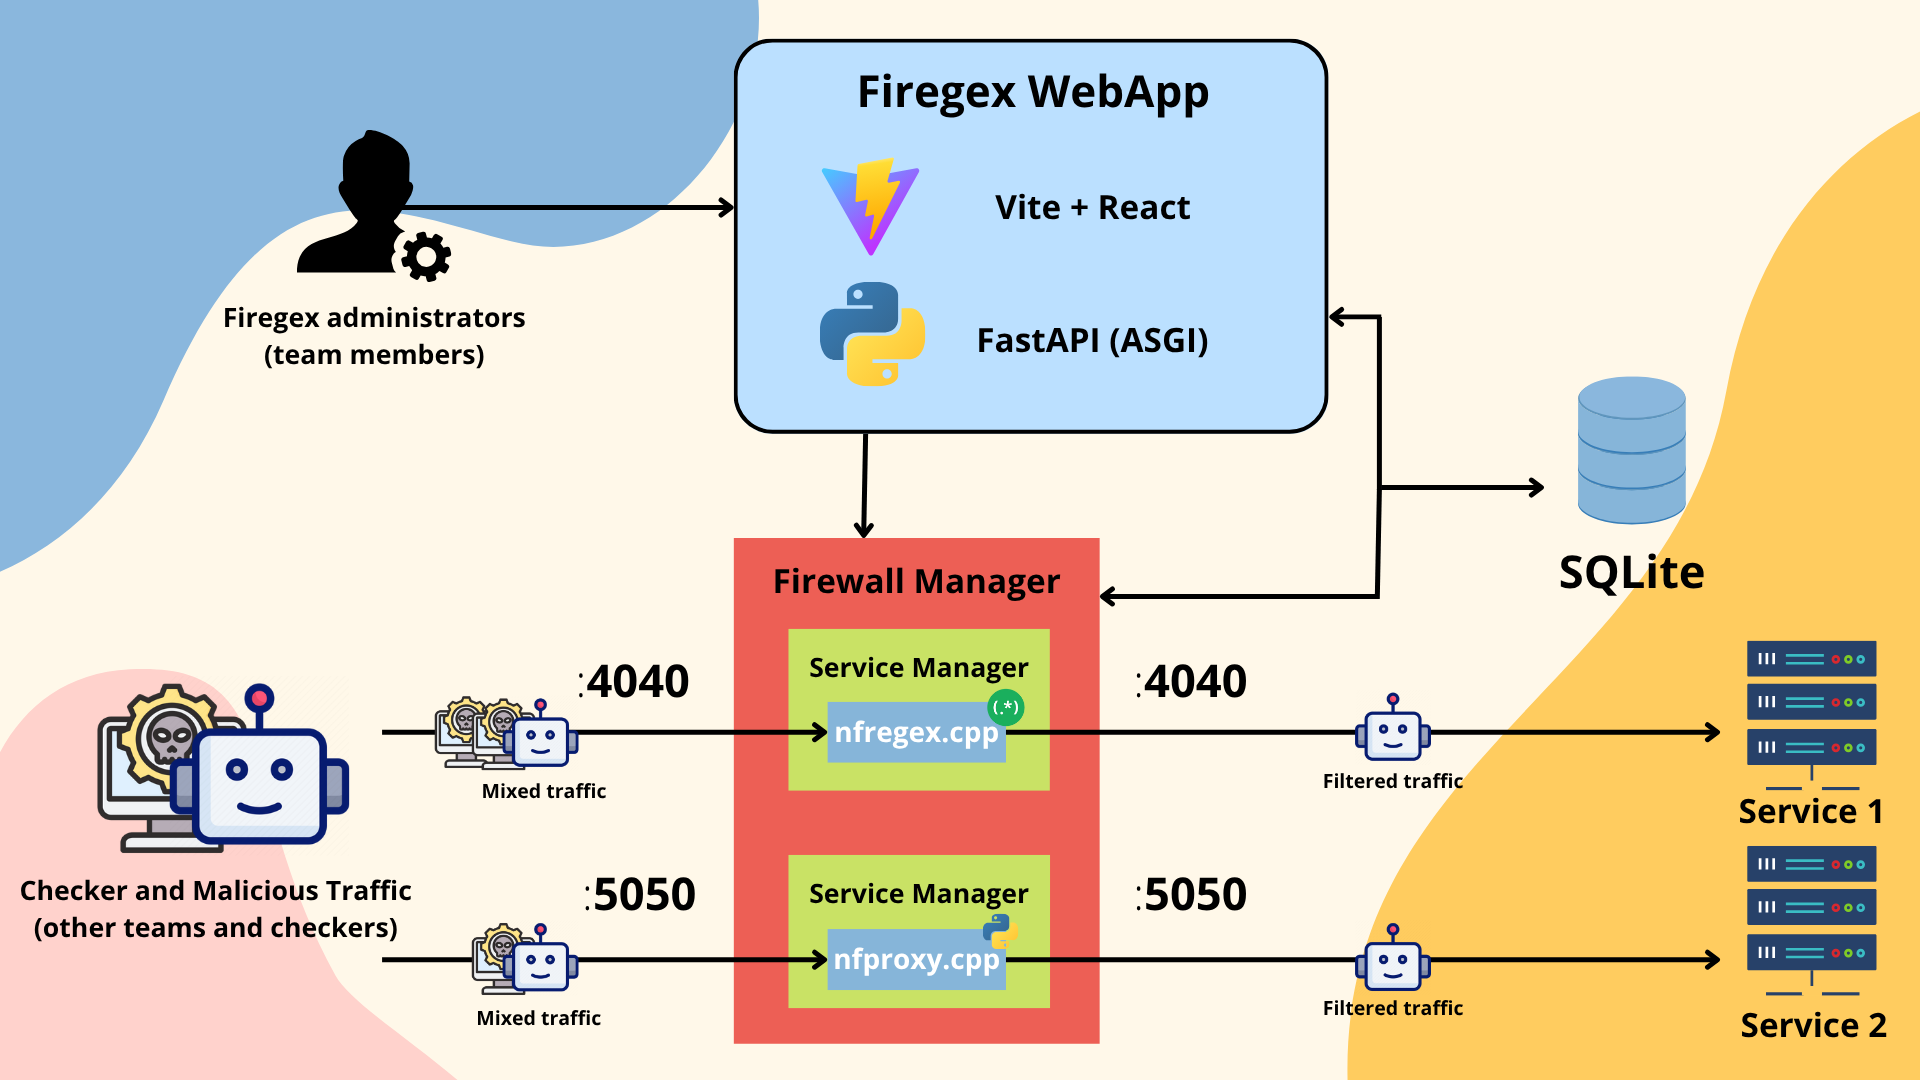
\includegraphics[width=0.98\textwidth]{images/chapter2/FiregexInternals.png}
    \caption{Schema generale dell'architettura di Firegex.}\label{fig:firegex_arch}
\end{figure}

Firegex, avendo un interfaccia web, è composto da un frontend scritto in react\footcite{\url{https://react.dev/}}{react} (usando vite\footcite{\url{https://vite.dev/}}{vite}) e un backend sviluppato con fastapi\footcite{\url{https://fastapi.tiangolo.com/}}{fastapi}. Il backend utilizza inoltre dei moduli scritti in C++ per le funzionalità più critiche, come per lo scambio dei pacchetti lato kernel e l'elaborazione in tempo reale delle espressioni regolari. Inoltre per funzionare, fa intenso utilizzo delle funzionalità di \gls{nftables}\footcite{\url{https://netfilter.org/projects/nftables/}}{nftables}, e di \gls{nfqueue}\footcite{\url{https://netfilter.org/projects/libnetfilter_queue/}}{netfilter_queue}. L'intera infrastruttura è avviata tramite docker\footcite{\url{https://www.docker.com/}}{docker} che ne permette un avvio immediato e senza configurare parametri: docker è usualmente lo strumento principale per l'avvio di servizi in competizioni \gls{ctf}, pertanto nella maggior parte dei casi è già presente e configurato correttamente. In Figura~\ref{fig:firegex_arch} è mostrato uno schema generale dell'architettura di Firegex.

\subsection{Frontend e Backend}
\begin{itemize}
    \setlength{\itemsep}{1pt}
    \setlength{\parskip}{1pt}
    \item \textbf{Frontend (React):} L'interfaccia utente risulta fortemente interattiva e intuitiva nelle fasi di creazione dei filtri, nel loro monitoraggio e la gestione degli stessi. L'interfaccia è parte fondamentale di Firegex, poiché consente di soddisfare uno dei punti chiave del progetto: la semplicità di utilizzo;
    \item \textbf{Backend (FastAPI + C++):} Il backend è realizzato utilizzando FastAPI, un framework python moderno e ad alte prestazioni per la creazione di \gls{api} \gls{http}, integrato con moduli critici scritti in C++. Questa combinazione consente di gestire le richieste in maniera estremamente veloce ed affidabile, garantendo al contempo, l'esecuzione delle operazioni critiche a livello di rete con le performance di un linguaggio a basso livello. Il backend inoltre svolge anche un ruolo attivo nell'applicazione delle regole di rete tramite il modulo ufficiale di libnftables\footcite{\url{https://git.netfilter.org/nftables/tree/py}}{nftables_python}.
\end{itemize}

\subsection{Moduli C++}
Le parti critiche di networking gestite da Firegex sono implementate in C++. I moduli di firegex che lo prevedono infatti, hanno un eseguibile compilato, responsabile del filtraggio, che si occupa di intercettare i pacchetti dal kernel Linux e di implementare la logica prevista dalla funzionalità per cui è stato realizzato. I moduli che attualmente fanno utilizzo di questi eseguibili sono \texttt{\gls{nfregex}} e \texttt{\gls{nfproxy}}. Essi fanno utilizzo di librerie aventi bassi tempi di elaborazione (permettendo alte prestazioni in rete) come libtins\footcite{\url{https://libtins.github.io/}}{libtins}, libmnl\footcite{\url{https://netfilter.org/projects/libmnl/}}{libmnl}, vectorscan\footcite{\url{https://vectorcamp.gr/project/vectorscan/}}{vectorscan} (specificatamente per \texttt{\gls{nfregex}}), e le C \gls{api} di python\footcite{\url{https://docs.python.org/3/c-api/}}{python_c_api} (specificatamente per \texttt{\gls{nfproxy}}). La scelta del linguaggio C++ ha permesso di perseguire i seguenti obiettivi:

\begin{itemize}
    \setlength{\itemsep}{1pt}
    \setlength{\parskip}{1pt}
    \item \textbf{Prestazioni elevate}: Grazie all'efficienza del linguaggio C++ e alla possibilità di gestire le interazioni a basso livello con il sistema operativo, il filtraggio del traffico avviene con latenze estremamente ridotte;
    \item \textbf{Parallelizzazione}: I filtri che richiedono elaborazione userspace facendo uso di \gls{nfqueue}, sono gestiti in un sistema di elaborazione multi-thread, garantendo una gestione ottimale del traffico in situazioni di carico elevato e con un numero di connessioni elevate;
    \item \textbf{Integrazione con librerie di rete}: L'utilizzo di librerie specializzate come libtins e libmnl (anch'esse scritte in C++), consente di implementare funzionalità avanzate mantenendo affidabilità su come vengono elaborati i pacchetti in rete, facendolo con un costo computazionale basso.
\end{itemize}

\section{Funzionalità}

All'interno di Firegex sono presenti attualmente quattro moduli principali, ognuno con delle funzionalità specifiche che permettono di applicare filtri con tecnologie e funzionalità differenti. I moduli sono \texttt{\gls{nfregex}}, \texttt{firewall}, \texttt{\gls{porthijack}} e \texttt{\gls{nfproxy}}. All'interno di questi moduli firegex possiede una documentazione interna alla piattaforma stessa che permette di comprendere come utilizzare le funzionalità offerte, e come configurare i filtri in maniera corretta.

Firegex è avviabile tramite un unico comando mostrato in Figura~\ref{lst:firegex_one_cmd}, supponendo che docker\footcite{\url{https://www.docker.com/}}{docker} sia stato già installato nel sistema.

\begin{listing}[H]
\begin{minted}[
    frame=single,
    framerule=0.8pt,
    fontsize=\footnotesize,
    breaklines
]{bash}
sh <(curl -sLf https://pwnzer0tt1.it/firegex.sh)
\end{minted}
\vspace{-1em}
\caption{One-Command per l'esecuzione di Firegex.}\label{lst:firegex_one_cmd}
\end{listing}

\subsection{Modulo nfregex}
Il modulo \texttt{\gls{nfregex}} (pensato originariamente come unico e principale) possiede funzionalità per la creazione di filtri basati su espressioni regolari. Utilizzando \gls{nfqueue} in combinazione con \gls{nftables}, questo modulo intercetta le richieste di rete direttamente a livello kernel. La funzionalità permette l'utilizzo di \gls{regex} \gls{pcre}\footcite{\url{https://www.pcre.org/}}{pcre_website} \textit{compliant} tramite l'utilizzo di vectorscan\footcite{\url{https://vectorcamp.gr/project/vectorscan/}}{vectorscan} (fork di hyperscan\footcite{\url{https://www.usenix.org/system/files/nsdi19-wang-xiang.pdf}}{wang2019hyperscan} compatibile con arm64) per garantire prestazioni elevate e una corretta elaborazione delle regole. La funzionalità supporta \gls{ipv4} e \gls{ipv6}, e protocolli di livello superiore come \gls{tcp} e \gls{udp}. Per i pacchetti \gls{tcp}, la \gls{regex} viene applicata all'intero flusso ricostruito e ordinato, tramite le stream \gls{regex} disponibili in vectorscan.

\subsection{Modulo firewall}
La funzionalità \texttt{firewall} di Firegex offre un controllo completo sul traffico di rete, tramite regole simili a quelle offerte da strumenti che agiscono a livello di rete e di trasporto come \gls{ufw} o iptables. Dispone quindi di funzionalità basilari e risulta utile per applicare questa tipologia di regole evitando ulteriori tool di filtering che potrebbero entrare in conflitto con firegex.

\subsection{Modulo porthijack}
Il modulo \texttt{\gls{porthijack}} introduce la capacità di reindirizzare il traffico destinato ad una determinata porta verso un’altra. Questa funzionalità è particolarmente utile in scenari dove si ha il bisogno di costruire un proxy personalizzato, ma si vuole evitare la riconfigurazione del servizio di base. \texttt{Porthijack} infatti consente di impostare un redirect del traffico dall'interfaccia su cui il servizio viene esposto nella rete di gara, dirottandolo per un proxy in \textit{localhost}, che poi tramite la stessa interfaccia di \textit{loopback} inoltrerà il traffico al servizio originale.

\subsection{Modulo nfproxy}
\texttt{\gls{nfproxy}}, il modulo trattato in questo lavoro di tesi, sfrutta le funzionalità di \texttt{\gls{nfqueue}} per l'intercettazione del traffico, simulando lato utilizzatore il comportamento di un tradizionale proxy python. Le caratteristiche principali del modulo sono:
\begin{itemize}
    \setlength{\itemsep}{1pt}
    \setlength{\parskip}{1pt}
    \item \textbf{Sviluppo in Python:} Permette agli sviluppatori di scrivere e integrare filtri personalizzati in linguaggio Python, offrendo un altissimo livello di flessibilità per l'analisi del traffico;
    \item \textbf{Parsing avanzato dei protocolli:} Tramite funzionalità predefinite è possibile eseguire la decodifica di protocolli come \gls{http}, in modo immediato e già disponibile all'utilizzo, senza che queste funzionalità debbano essere implementate manualmente;
    \item \textbf{Test e validazione:} I filtri possono essere provati in anticipo tramite il comando fgex, rendendo possibile la prova del filtro prima si applicarlo al traffico;
    \item \textbf{Interfaccia grafica:} L'interfaccia di dettaglio del servizio permette di visualizzare in tempo reale i log e le eventuali eccezioni che si verificano durante l'esecuzione del filtro.
\end{itemize}

Il seguente modulo è stato introdotto in vista di scenari complessi dove gli elementi da individuare per il corretto filtraggio non sono facilmente individuabili tramite \gls{regex}. In Figura~\ref{fig:nfproxy_interface} si mostra l'interfaccia grafica realizzata per il modulo \texttt{nfproxy}.

\begin{figure}[H]
    \centering
    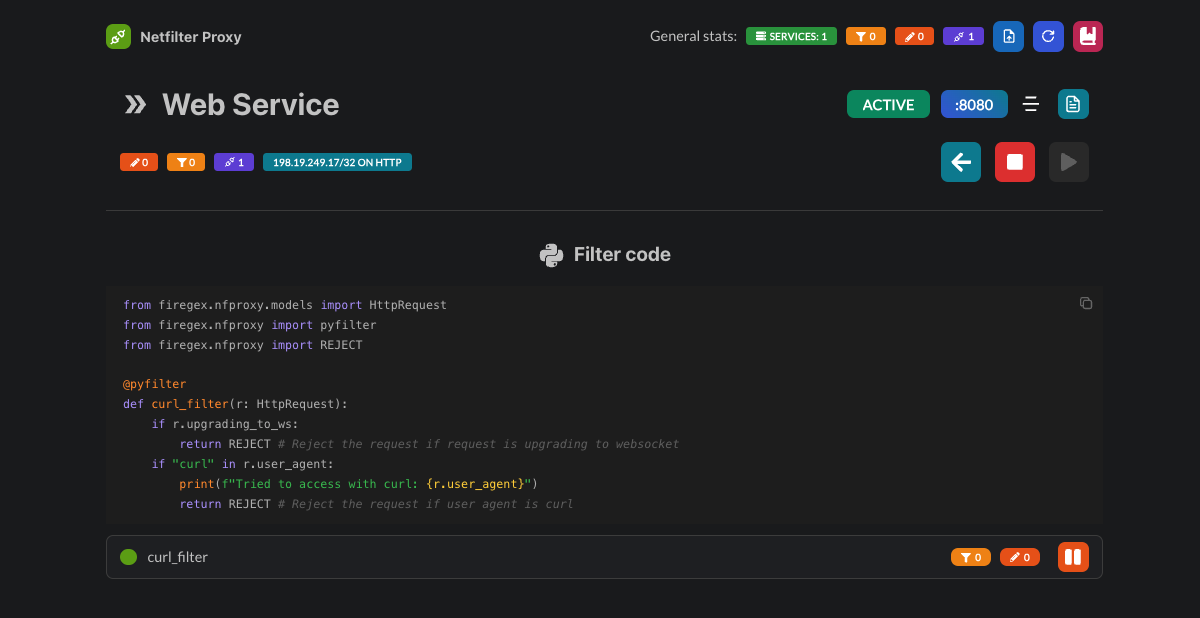
\includegraphics[width=0.98\textwidth]{images/chapter2/NFProxyInterface.png}
    \caption{Interfaccia di dettaglio del servizio nel modulo nfproxy.}\label{fig:nfproxy_interface}
\end{figure}

Nei prossimi capitoli verrà trattato in dettaglio \texttt{\gls{nfproxy}} con le sue funzionalità, le problematiche affrontate e le soluzioni adottate.
